\documentclass[12pt]{article}
\usepackage[margin=1in]{geometry}
\usepackage{natbib}
\usepackage{graphicx}
\usepackage{amsmath}
\usepackage{float}
%\bibliographystyle{plain}

\title{ASTR 565 \\
Computer Problem 3: Convection and Radiation Zones in Main Sequence
Stars}
\author{Laurel Farris}
\date{03 November 2015}
\begin{document}
\maketitle

\section{Introduction}
Energy is transferred through the interior of stars by means of three
primary mechanisms: radiation, conduction, and convection. The
efficiency of this transfer depends on the temperature gradient, one
of the fundamental equations of stellar structure.
Convection
 arises due to instabilites in stellar interiors;
 if a parcel of gas is displaced and its
mass density is less than that of its surroundings,
the blob will continue to rise, and this is convection.\\

\noindent
If the pressure balance between the blob and its surroundings adjusts
itself on much shorter timescales than the temperature (due to
acoustic waves traveling through this region), the displacements are
adiabatic.\\
%\cite{something} !!! acoustic waves!!!

%\noindent Much of the criteria for convective instability in stars comes from
%the \textit{Mixing Length Theory}, or MLT \cite{Mikes}.\\

\noindent
While convection is not well understood, there
are several constraints that can be place on when and where this
phenomenon occurs in a range of stellar masses.
One of these is
$\nabla$, defined as
 \begin{equation}
    \nabla \equiv \frac{dln T}{dlnP} = -\frac{r^2P}{Gm\rho}
    \frac{1}{T}\frac{dT}{dr}
 \end{equation}
This is the true driving gradient of the star, and is determined by
the
mechanism that is driving the luminosity to escape. If this mechanism
happened to be radiative transport only, then $\nabla$ would be equal
to the radiative gradient, $\nabla_{rad}$, defined as
\begin{equation}
    \nabla_{rad} \equiv \Big(\frac{dlnT}{dlnP}\Big)_{rad}
    = -\frac{3}{16\pi acG}
    \frac{P\kappa_R}{T^4}\frac{L}{m}
\end{equation}
This gradient is required for a purely
radiative region. If $\nabla_{rad}$ is
greater than $\nabla$, then $\nabla$ is not steep enough to transport the
energy and an additional mechanism is required to drive the
radiation outward.\\

\noindent
This leads us to the third gradient, the adiabatic gradient,
$\nabla_{ad}$, defined as
\begin{equation}
    \nabla_{ad} \equiv \Big(\frac{dlnT}{dlnP}\Big)_{ad}
    = \frac{\Gamma_2-1}{\Gamma_2}
\end{equation}
The condition for instability is the
\textbf{Schwarzschild criterion}: $\nabla > \nabla_{ad}$;
if the temperature gradient is not steep enough to carry luminosity
through radiative transport, convection is required to do so.\\

\noindent
Another way to model convection is through the
Brunt-V$\ddot{\rm a}$is$\ddot{\rm a}$l$\ddot{\rm a}$
frequency (N$^2$):
\begin{equation}
    N^2 = g\Big(\frac{1}{\gamma P}\frac{dP}{dr} -
    \frac{1}{\rho}\frac{d\rho}{dr}\Big)
\end{equation}
or, in terms of the temperature gradients:
\begin{equation}
    N^2 = \frac{g^2\rho}{P}(\nabla_{ad} - \nabla + \nabla_{\mu})
\end{equation}
where $\nabla_{\mu}$ is the composition gradient.
Temporarily ignoring $\nabla_{\mu}$ (which is effectively zero in
convective regions; the mixing of materials results in a constant mean
molecular weight), one can see that N$^2$ will be
negative when the criteria for instability holds ($\nabla >
\nabla_{ad}$), indicating convection.
However, it is possible for $\nabla_{\mu}$ to be large enough
to cause N$^2$ to be positive, resulting in a medium that is stable,
even though it satisfies the Schwarzchild criterion.
When this happends, the region satisfies the
\textit{Ledoux criterion}, resulting in \textit{semiconvection}, or
weak convection. Physically, blobs of material
are subject to oscillation about a point in their static environment,
but are stable to large-scale convection.

\section{Methods}
To explore the variation in location and depth of convection zones for
main sequence stars, MESA was used to produce models for 19 stars
 with initial masses ranging
from 1.3 M$_\odot$ to 20 M$_\odot$.
An HR diagram showing the final stage for each model (where the hydrogen
mass fraction dropped to 0.35) is shown in figure \ref{hr_diagram}.\\

\begin{figure}
  \centering
  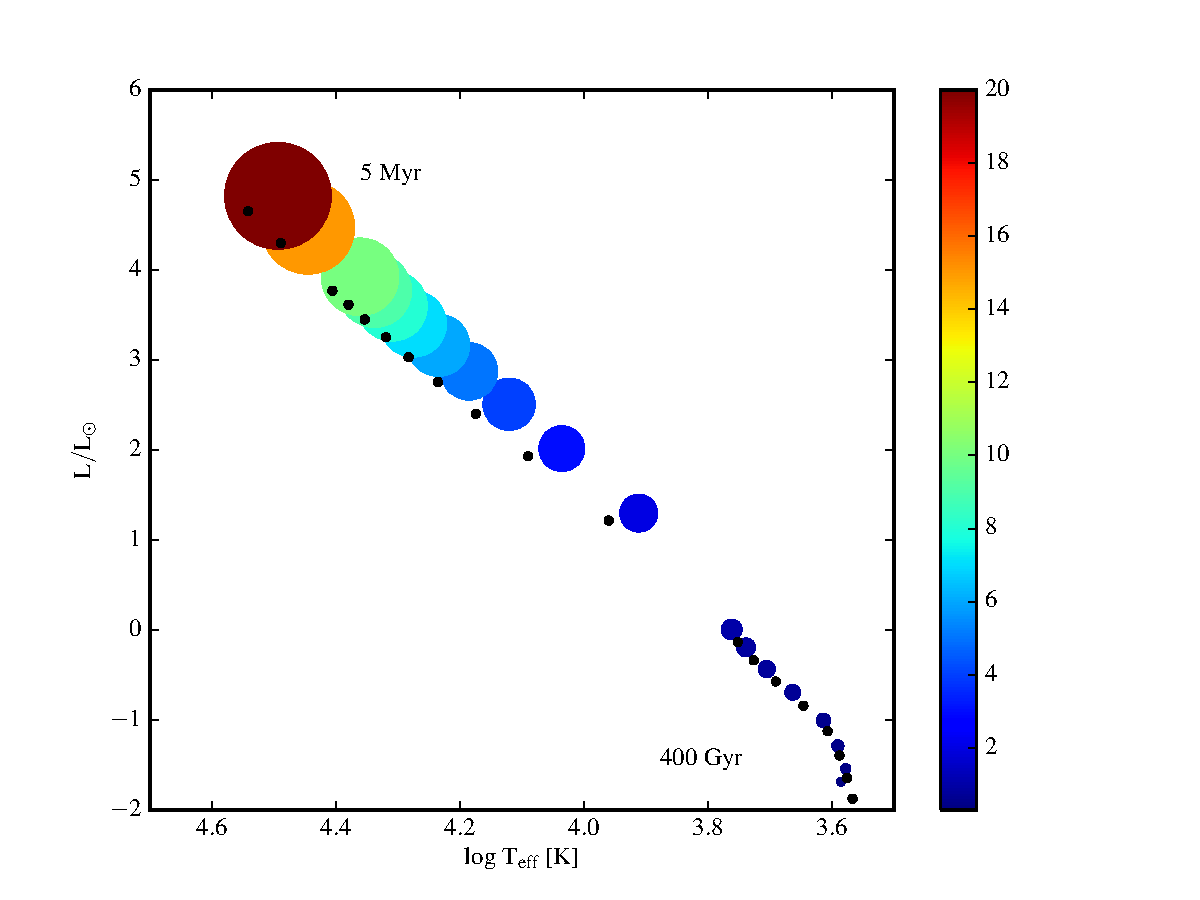
\includegraphics[width=7.0in]{hr_diagram.pdf}
  \caption{HR-Diagram of all models at both the ZAMS
  (black dots) and their final positions upon reaching a hydrogen mass
  fraction of 0.35. The final radius of each star is plotted to scale by
  size, and the color is an indication of the final mass (in units of
  M$_{\odot}$). The final age
  is displayed for highest (20 M$_{\odot}$) and lowest (0.3
  M$_{\odot}$) mass stars for comparison. The ZAMS points are not
  scaled.}
  \label{hr_diagram}
\end{figure}

\noindent
 Each of the gradients described in the introduction is
available as output in MESA, as well as the
Brunt-V$\ddot{\rm a}$is$\ddot{\rm a}$l$\ddot{\rm a}$
frequency,
 so these values were used to determine where
 the convection boundaries might be for each model.
 Since the criteria for instability ($\nabla > \nabla_{ad}$) can be met
 and still only result in a region that is semi-convective, as discussed
 above, the sign of the
Brunt-V$\ddot{\rm a}$is$\ddot{\rm a}$l$\ddot{\rm a}$
frequency (negative)
 was used to determine where large scale convection was taking place.
The results of these data for each model
are shown in figures \ref{money} and
\ref{money2}, where figure \ref{money} shows the convective boundaries as a
function of mass ratio, and figure \ref{money2} shows the convective
boundaries as a function of radius. Once the endpoints of region were found,
a cubic interpolation was applied to make these boundaries continuous across
all masses between 0.3 M$_{\odot}$ and 20 M$_{\odot}$.\\

\noindent
Also shown in the figures is
where the dominant nuclear burning process (proton-proton chain or CNO cycle)
is taking place in the non-convective interiors. Both processes were also
contained in output variables from MESA (pp and cno), but determining the location
where each one takes place was not as straight-forward as simply using the sign
of the numbers. If the ratio of cno to pp was greater than 1, the CNO cycle
was assumed to be the dominant reaction taking place. However, the pp values
were always greater than zero (though not always by much, as they could get
as low as $\sim$ 10$^{-30}$). The values did increase substantially around
1.0, so anything greater than this was determined to be a dominant process.
\newpage
% Money plot!
\begin{figure}
  \centering
  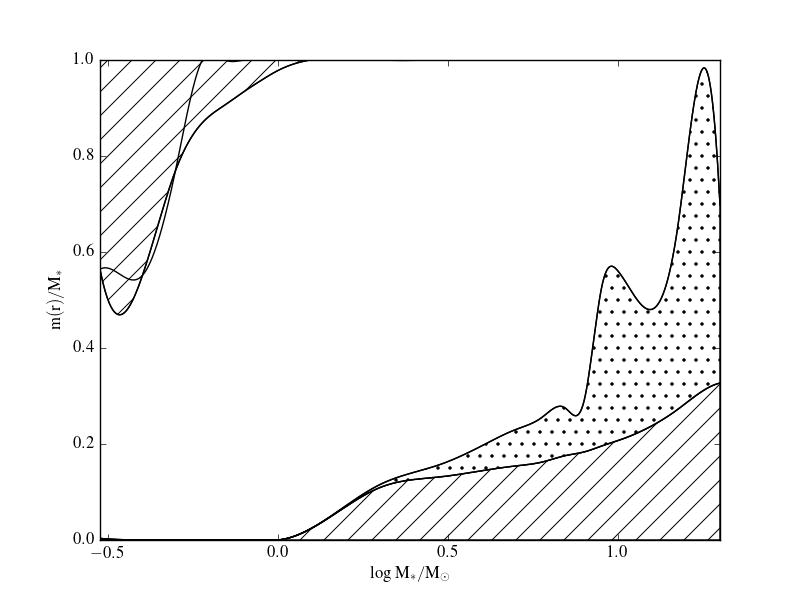
\includegraphics[width=7.0in]{money.png}
  \caption{This plot shows where the convection zone boundaries of
  each model occur according to the mass fraction of the entire star.
  The hatched areas show the location of the convection zones,
  the dotted areas are where the CNO cycle is taking place, and the
  other areas are where the proton-proton chain is taking place.}
  \label{money}
\end{figure}
\newpage
% Money plot again!
\begin{figure}
  \centering
  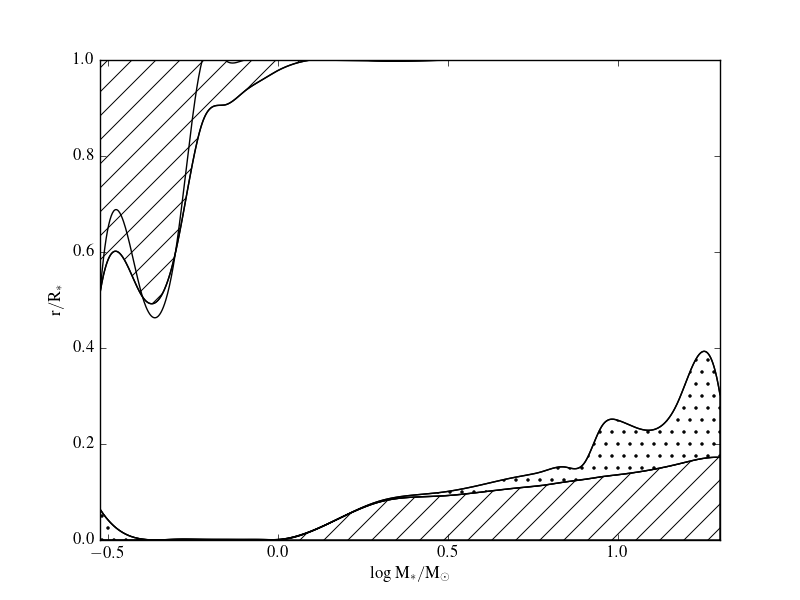
\includegraphics[width=7.0in]{money2.png}
  \caption{This is the same as figure \ref{money}, but with the
  boundaries shown according to their radial value (as a fraction of
  each star's total radius).}
  \label{money2}
\end{figure}
\newpage
\noindent


% 4 - 7
\noindent
For further analysis, the gradients for the 0.3 M$_{\odot}$ star
and the 10 M$_{\odot}$ were plotted as functions of temperature, as a
comparison between convective behavior in low and high mass stars.
The results are shown in figures \ref{littlegrad} and \ref{biggrad}.
For these same two models, the
Brunt-V$\ddot{\rm a}$is$\ddot{\rm a}$l$\ddot{\rm a}$
frequency was also plotted as a function of temperature
to examine areas of semi-convection. These results are shown in
figures \ref{littleBV} and \ref{bigBV}.

\section{Results}
The first thing that is immediately apparent
upon examination of figures \ref{money} and \ref{money2}, is that
the variation of convective boundaries with stellar mass across the
range of models is much different than the variation with
stellar radius.
%In our sun, for instance, the convection zone extends
%from near the surface to a depth of almost halfway into the star, yet
%this region is only a small fraction of the total solar mass.
Low mass stars are known to be fully convective due to larger
opacities, so we would expect figure \ref{money2} to show convection
throughout the majority of the radius (unfortunately, due to an
unknown
programming error, the plot does not follow the correct trend for low
mass stars).\\

\noindent
The low mass model can be further explained
in figure \ref{littlegrad}, where the radiative gradient
for the 0.3 M$_{\odot}$ model
is much higher than the adiabatic and true
gradients. As discussed above, this implies that the true driving
gradient of the star is not steep enough to transport the luminosity
by radiation alone. This only ceases to be the case in the hottest
region of the star, where $\nabla_{rad}$ briefly drops below the other
two. This corresponds to where the
Brunt-V$\ddot{\rm a}$is$\ddot{\rm a}$l$\ddot{\rm a}$
frequency
is positive for this model, as shown in figure \ref{littleBV}. \\

\noindent
For the higher mass models (greater than or equal to 1M$_{\odot}$), a
convective core appears to emerge in figures \ref{money} and ref{money2},
as we would expect. Convection in
the outer regions extends to shallower depths as the temperature
increases, and as can also be seen in the figures
, the outer convection region practically disappears at
the surface. Contrary to the gradients for the 0.3 M$_{\odot}$ model, the
radiative gradient for the 10 M$_{\odot}$ model (figure \ref{biggrad})
is lower than the adiabatic,
except in the deepest regions, where core convection takes place for
high mass stars, and a few places closer to the surface. Between these
two regions is where the
Brunt-V$\ddot{\rm a}$is$\ddot{\rm a}$l$\ddot{\rm a}$
has positive values, as shown in figure \ref{bigBV}. The spikes at the
edges occur near the boundaries of the convection zones discussed
above, and the inner region of the high-mass model shows varying
degrees of semi-convection. \\

\noindent
To obtain a more quantitative idea of why convection takes place where it
does (particularly for the 0.3 M$_{\odot}$ and 10 M$_{\odot}$
models as investigated here,
equation (2) can be rewritten as
\begin{equation}
  \nabla_{rad} = \frac{3k_B}{16\pi acGm_u}\frac{\kappa}{\mu}
                 \frac{L}{m}\frac{\rho}{T^3}
\end{equation}
where it is easier to see that a high value of
$\nabla_{rad}$ can arise from $\frac{L}{m}$,
 $\kappa$, and/or $\rho/T^3$ being large.
The opacity ($\kappa$) is definitely larger for lower mass stars,
where their surface temperatures are cooler, and thus $\rho/T^3$
can also get quite large.\\

\begin{figure}
  \centering
  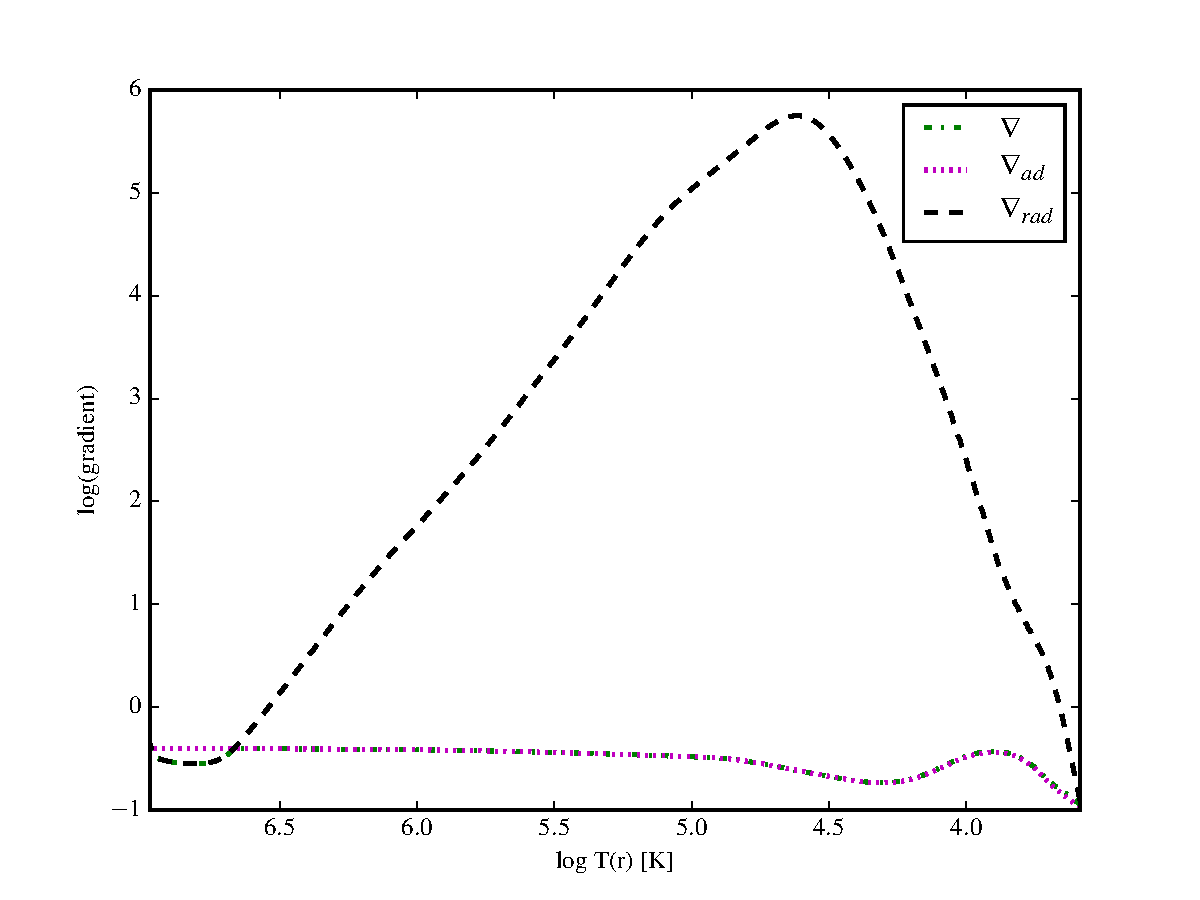
\includegraphics[width=7.0in]{littlegrad.pdf}
  \caption {This plot shows the temperature gradient ($\nabla$),
  the adiabatic gradient ($\nabla_{ad}$), and the radiative gradient
  ($\nabla_{rad}$) for a 0.3 M$_{\odot}$ model as functions of
  (decreasing) temperature.}
  \label{littlegrad}
\end{figure}
\begin{figure}
  \centering
  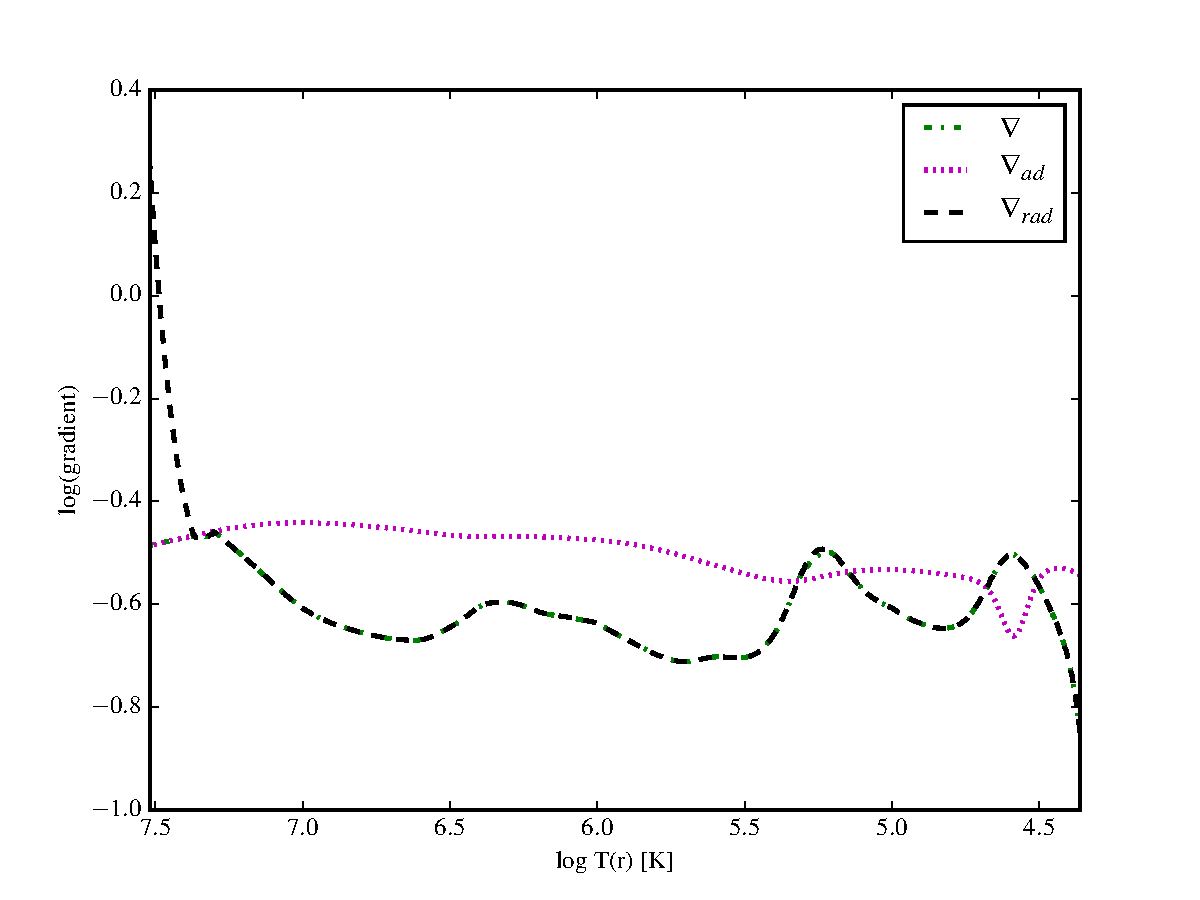
\includegraphics[width=7.0in]{biggrad.pdf}
  \caption {This plot shows the temperature gradient ($\nabla$),
  the adiabatic gradient ($\nabla_{ad}$), and the radiative gradient
  ($\nabla_{rad}$) for a 10 M$_{\odot}$ model as functions of
  (decreasing) temperature.
  }
  \label{biggrad}
\end{figure}
\begin{figure}
  \centering
  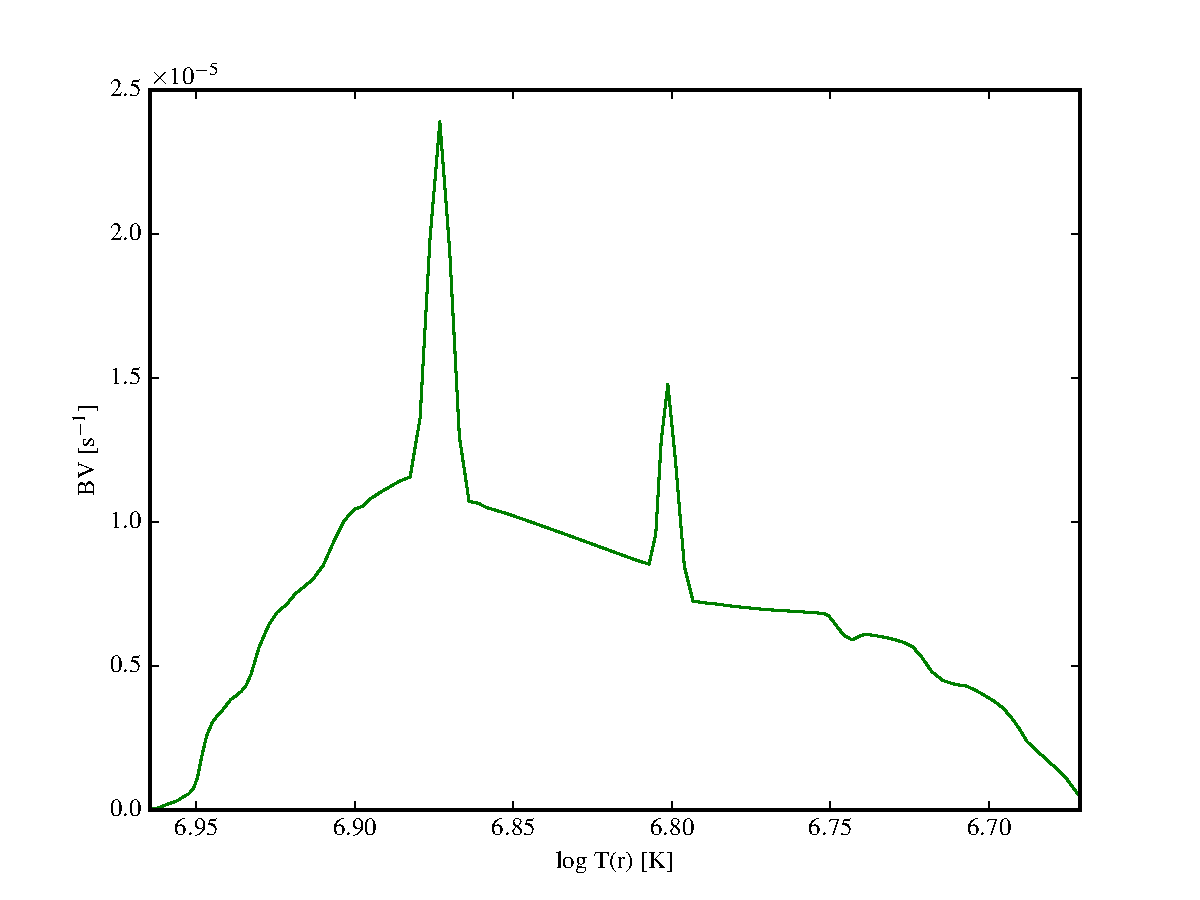
\includegraphics[width=7.0in]{littleBV.pdf}
  \caption{This plot shows the
  Brunt-V$\ddot{\rm a}$is$\ddot{\rm a}$l$\ddot{\rm a}$
  frequency (N$^2$) for a
  0.3 M$_{\odot}$ model as a function of (decreasing)
  temperature. }
  \label{littleBV}
\end{figure}
\begin{figure}
  \centering
  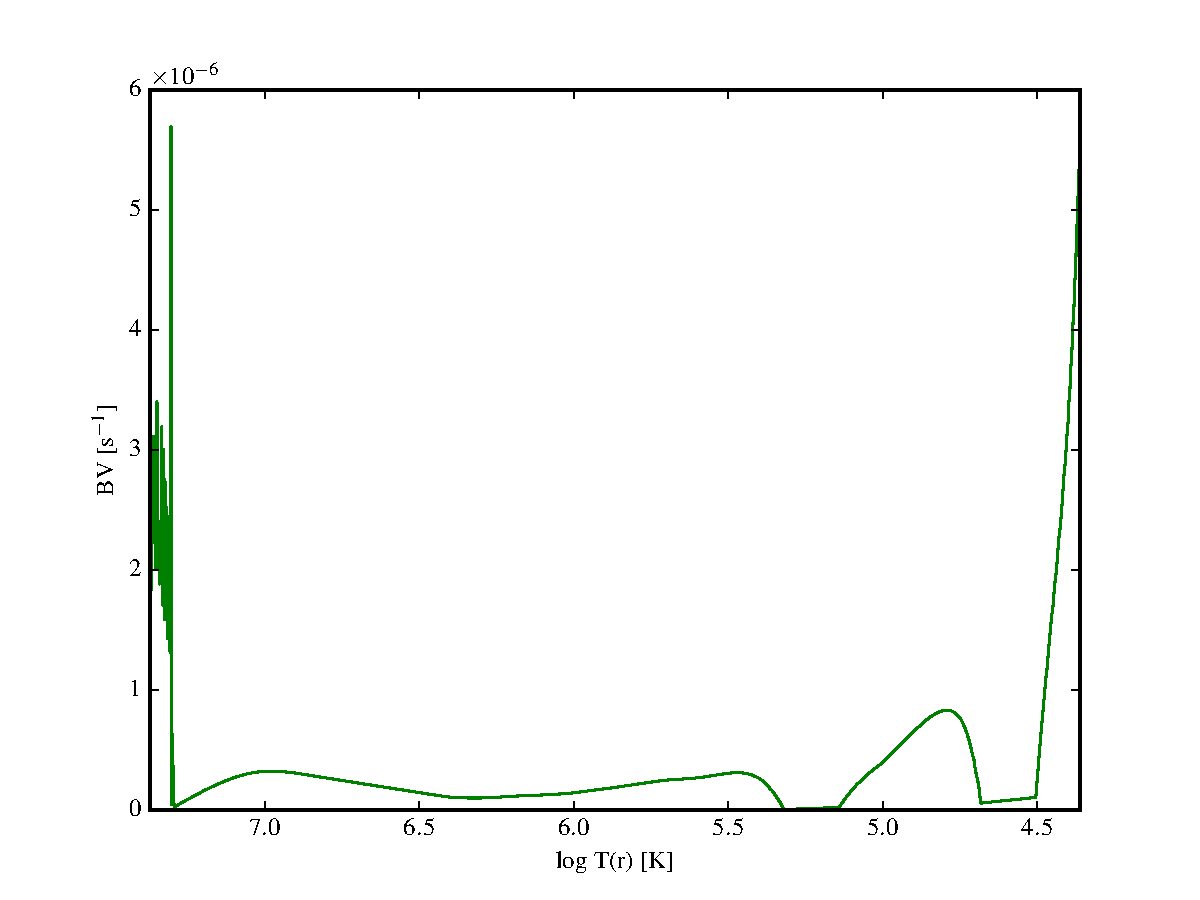
\includegraphics[width=7.0in]{bigBV.pdf}
  \caption{This plot shows the
  Brunt-V$\ddot{\rm a}$is$\ddot{\rm a}$l$\ddot{\rm a}$
  frequency (N$^2$) for a 10 M$_{\odot}$ model as a function
  of (decreasing) temperature.}
  \label{bigBV}
\end{figure}

\section{Conclusions}
Low mass stars tend to have high opacities in their outer regions,
which can lead to convection, whereas high mass stars have a high
energy generation rate, leading to convection in their cores. This is
illustrated plainly in figures \ref{money} and \ref{money2}, but
doesn't explain the small convection areas in the outermost regions of
the high mass stars. In figure \ref{biggrad}, the different between
$\nabla_{ad}$ and $\nabla_{rad}$ oscillates back and forth a couple
times, illustrating the convective inconsistency in the lower
temperature regions (outer layers).
The Brunt-V$\ddot{\rm a}$is$\ddot{\rm a}$l$\ddot{\rm a}$
frequency for the 0.3 M$_{\odot}$ star has a
positive value between temperatures of about 4.5 MK and 9 MK.
The slope of the line is fairly smooth, except for two significant
spikes around temperatures of 7.5 MK and a smaller one at 6.3 MK.
Since the ratio $\rho/T^3$ can result in convection if it gets large
enough, this may suggest a low enough density at those temperatures
for partial displacement of material, but not low enough to become
completely unstable.


%\bibliography{reffile}
\end{document}


